\documentclass{beamer}
\usetheme{default}
\usepackage{tikz}
\usetikzlibrary{arrows}
\begin{document}

\begin{frame}{Background}

A Markov Decision Process (MDP) is a 4 tuple where:
\begin{itemize}
\item $S$ is a finite set of states
\item $A$ is a finite set of actions
\item $P_a(s,s')$ is the probability that taking action $a$ in state $s$ at time $t$ will lead to state $s'$ at time $t+1$.
\item $R_a(s,s')$ is the immediate reward received after transition from state $s$ to state $s'$
\end{itemize}

The goal of an agent in an MDP is to maximize long term expected rewards. 

\end{frame}


\begin{frame}{Graph}

Representing an MDP over undirected edges:

\makebox[\textwidth][c]{
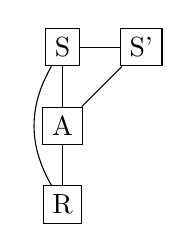
\begin{tikzpicture}[scale=.5,every node/.style={rectangle,draw}]
  \node (n6) at (1,5) {S};
  \node (n4) at (1,3) {A};
  \node (n5) at (3,5) {S'};
  \node (n1) at (1,1) {R};

  \path[every node/.style={font=\sffamily\small}]
    (n6) edge (n4)
         edge (n5)
         edge [bend right] (n1)
    (n4) edge (n1)
         edge (n5);
\end{tikzpicture}}
Where each node in \{S,A,R,S'\} may be decomposed into many nodes with connections between groups but not with a group. 

\makebox[\textwidth][c]{
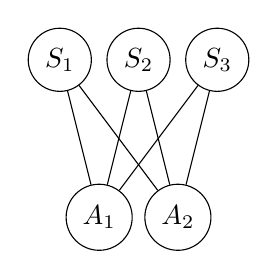
\begin{tikzpicture}[scale=.5,every node/.style={circle,draw}]
  \node (s1) at (1,5) {$S_1$};
  \node (s2) at (3,5) {$S_2$};
  \node (s3) at (5,5) {$S_3$};
  \node (a1) at (2,1) {$A_1$};
  \node (a2) at (4,1) {$A_2$};

  \path[every node/.style={font=\sffamily\small}]
    (s1) edge (a1)
         edge (a2)
    (s2) edge (a1)
         edge (a2)
    (s3) edge (a1)
         edge (a2);

\end{tikzpicture}}
Note this graph is not triangulated -- can you see why?
\end{frame}

\begin{frame}{Exponential Family}
Sufficient statistics are indicator functions defined over the nodes and edges, yielding the following exponential family:
$$
p(x;\theta)
=
exp\left\{\sum_{s \in V}\theta_{sj}(X_s) + \sum_{(s,t) \in E} \theta_{stjk}(X_s,X_t) - A(\theta)\right\}
$$
\end{frame}

\begin{frame}{Domain - 9x9 Gridworld}
\makebox[\textwidth][c]{
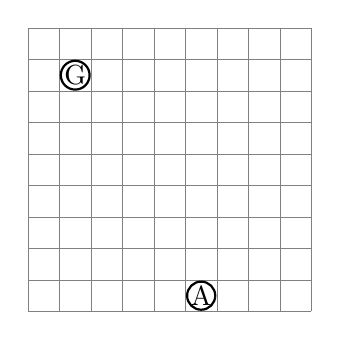
\begin{tikzpicture}[scale=.4,inner sep=0pt,thick,
    dot/.style={fill=blue,circle,minimum size=3pt}]
    \draw[help lines] (0,0) grid (9,9);
    \node[circle,draw] at (5.5,.5) {A};
    \node[circle,draw] at (1.5,7.5) {G};
\end{tikzpicture}}

\begin{itemize}
\item There are 9 state binary state variables associated with the X coordinate and 9 associated with the Y coordinate of the agent. At any position one X and one Y variable are True.
\item Two binary variables determine which of the 4 direcitonal actions ($\leftarrow,\rightarrow,\uparrow,\downarrow$) is taken.
\item A single reward node indicates whether or not the goal has been reached.
\item $|V|$ = 39; $|E|$ = 416; $|\theta| = |\phi|$ = 1742
\end{itemize}
\end{frame}

\begin{frame}{Learning}
Given the graph and some set of sample data $\textrm{T}$, the objective is to find $\theta$ maximing the empirical likelihood:

\[
\arg\max_\theta \left\{
  \frac{1}{\textrm{T}}\sum_{t=1}^{\textrm{T}}p(X^t|\theta,G)
\right\}
\]

It is intractable to compute $A(\theta)$ and MLE cannot be used since the graph is not triangulated. Therefore the pseudo-likelihood is used:

\[
  \tilde{p}(X|\theta,G) = \prod_{s=1}^p p(x_s | x_{V\setminus s})
\]

where

\[
p(x_s | x_{V\setminus s})
=
\frac{exp\{\theta^\intercal\phi(X)\}}{\sum_{j \in \chi} exp\{\theta^\intercal\phi(x_s = j | x_{V\setminus s})\}}
\]
\end{frame}


\begin{frame}{Theano}
\begin{itemize}
\item Now that the likelihood can be approximated efficiently, the remaining challenge is to find $\theta$ maximizing this likelihood. Because of the high dimensionality of the parameter space, the gradient of the objective function is required for tractable learning.
\item Theano (http://deeplearning.net/software/theano/) is a software packaged capable of taking analytic gradients of functions.
\item Combining the Theano-gradient of the pseudo-likelihood with conjugate descent software (http://docs.scipy.org/doc/scipy/reference/optimize.html) yields tractable learning.
\end{itemize}
\end{frame}

\begin{frame}{Results}

Data was generated by an optimal policy on the 9x9 Gridworld.

\begin{tikzpicture}[scale=.8]
 \definecolor{r1}{RGB}{0,129,188}
 \definecolor{r2}{RGB}{252,177,49}
 \definecolor{r3}{RGB}{35,34,35}
 \definecolor{r4}{RGB}{0,157,87}
 \definecolor{r5}{RGB}{238,50,78}
 \begin{scope}
   \clip (-6,2) rectangle (6,-.9);
   \foreach \col/\xp/\yp in {
     r5/4/0, r4/2/-1.8, r3/0/0,
     r2/-2/-1.8, r1/-4/0
   } {
     \path[draw=white,line width=.08cm,
     fill=\col,even odd rule]
     (\xp, \yp) circle (1.9cm)
     (\xp, \yp) circle (1.5cm);
   }
 \end{scope}
 \begin{scope}
   \clip (-6,-.9) rectangle (6,-3.8);
   \foreach \col/\xp/\yp in {
     r1/-4/0, r2/-2/-1.8, r3/0/0,
     r4/2/-1.8, r5/4/0
   } {
     \path[draw=white,line width=.08cm,
     fill=\col,even odd rule]
     (\xp, \yp) circle (1.9cm)
     (\xp, \yp) circle (1.5cm);
   }
 \end{scope}
\end{tikzpicture}
\end{frame}




\begin{frame}{Future Work - Control}
\begin{itemize}
\item In the control problem, agent must select the values of the action nodes. 
\item Objective: Use the learned $\theta$s to select actions mimicking the policy from which the data was generated.
\item Given an observed state, the goal is to find the \textit{most likely} configuration of the action nodes.
\item In other words, find the MAP configuration of action nodes given the observed state nodes.
\end{itemize}
\end{frame}

\end{document}
